\section{Brugsscenarier}
\label{TestAfSkalaBrugsscenarier}
%
Den eneste ændring, der er til brugsscenarierne, er når testpersonerne skal vælge destination, hvor antallet af afgange er ændret fra fire til fem, for at tilpasse destinationerne efter de reelle afgange, der er på den pågældende dag, hvor evalueringen udføres. De fem destinationer de rejsende kan vælge imellem fremgår af højre side på \autoref{fig:TilpassetDestination}, hvor venstre side gengiver skærmbilledet fra feltundersøgelsen. Undervejs som tiden går vil afgangene blive opdateret, så de passer med oversigtstavlerne.
%
\begin{figure}[H]
\centering
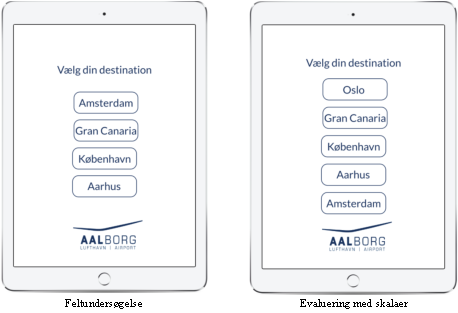
\includegraphics[width =0.7\textwidth]{Figure/TestdesignEvaluering/TilpassetDestination} 
\caption{Illustration af ændringerne foretaget fra feltundersøgelsen (venstre) til evalueringen med skalaerne (højre).}
\label{fig:TilpassetDestination}
\end{figure}
\noindent
%
Udover ændringen i hvilke destinationer, der kan vælges, er informationen til den specifikke destination ligeledes tilpasset så det svarer til informationerne fundet på Aalborg Lufthavns hjemmeside gældende for den 01/12-2017. 